\section{Kết quả thực hành và bằng chứng
chạy}\label{kux1ebft-quux1ea3-thux1ef1c-huxe0nh-vuxe0-bux1eb1ng-chux1ee9ng-chux1ea1y}

\subsection{Kiến trúc B0--B3}\label{kiux1ebfn-truxfac-b0b3}

Các số dưới được lấy từ mas\_benchmark.csv. Mỗi hệ chạy 11 ca, lặp 20
lần. Success có tính cả trạng thái từ chối đúng; tỷ lệ không đồng nghĩa
tỷ lệ yêu cầu có gợi ý sản phẩm.

{\def\LTcaptype{none} % do not increment counter
\begin{longtable}[]{@{}llllll@{}}
\toprule\noalign{}
Hệ & Success (\%) & P50 ms & P95 ms & Message/request & Violation
(\%) \\
\midrule\noalign{}
\endhead
\bottomrule\noalign{}
\endlastfoot
B0\_single & 100.00 & 0.0048 & 0.0090 & 0.00 & 0.00 \\
B1\_rule\_MAS & 100.00 & 0.2406 & 11.0973 & 6.00 & 0.00 \\
B2\_learned\_MAS & 100.00 & 0.3104 & 11.4029 & 6.00 & 0.00 \\
B3\_no\_validation & 72.73 & 0.2172 & 11.3042 & 4.73 & 18.18 \\
\end{longtable}
}

Không so tỷ lệ tốc độ B0/B1 trên các ca lỗi: baseline đơn trả trạng thái
timeout được tiêm đồng bộ, còn MAS chờ deadline thực. Phần learned
routing trong benchmark luôn nhận một câu ecommerce cố định, nên chỉ
phản ánh overhead tích hợp. Đánh giá đa miền nằm ở bảng classifier
riêng.

\subsection{Chỉ số classifier trên held-out
test}\label{chux1ec9-sux1ed1-classifier-truxean-held-out-test}

{\def\LTcaptype{none} % do not increment counter
\begin{longtable}[]{@{}lllll@{}}
\toprule\noalign{}
Lớp & Precision & Recall & F1 & Số câu \\
\midrule\noalign{}
\endhead
\bottomrule\noalign{}
\endlastfoot
ecommerce & 1.0000 & 1.0000 & 1.0000 & 36 \\
tourism & 1.0000 & 1.0000 & 1.0000 & 36 \\
healthcare admin & 1.0000 & 1.0000 & 1.0000 & 36 \\
\end{longtable}
}

Accuracy: 1.0000; macro-F1: 1.0000; threshold 0.5; coverage 1.0000. Tập
train, validation và test: 270, 54 và 108 câu. Vocabulary 79; seed 42.

\subsection{Ngoài miền: những lỗi cần giữ lại để phân
tích}\label{ngouxe0i-miux1ec1n-nhux1eefng-lux1ed7i-cux1ea7n-giux1eef-lux1ea1i-ux111ux1ec3-phuxe2n-tuxedch}

{\def\LTcaptype{none} % do not increment counter
\begin{longtable}[]{@{}lll@{}}
\toprule\noalign{}
Câu thử & Kết quả & Confidence \\
\midrule\noalign{}
\endhead
\bottomrule\noalign{}
\endlastfoot
xin chào & clarify & 0.4943 \\
thời tiết hôm nay thế nào & ecommerce & 0.9877 \\
viết thơ cho tôi & clarify & 0.6866 \\
giải phương trình & tourism & 0.9311 \\
cảm ơn bạn & clarify & 0.4943 \\
abc xyz & clarify & 0.4943 \\
\end{longtable}
}

Có 4/6 câu được từ chối và 2/6 bị nhận nhầm vào miền dù confidence cao.
Sáu câu là probe nhỏ, không phải một benchmark OOD đại diện. Không dùng
tỷ lệ này để ước lượng lỗi trên mọi yêu cầu người dùng.

\begin{center}
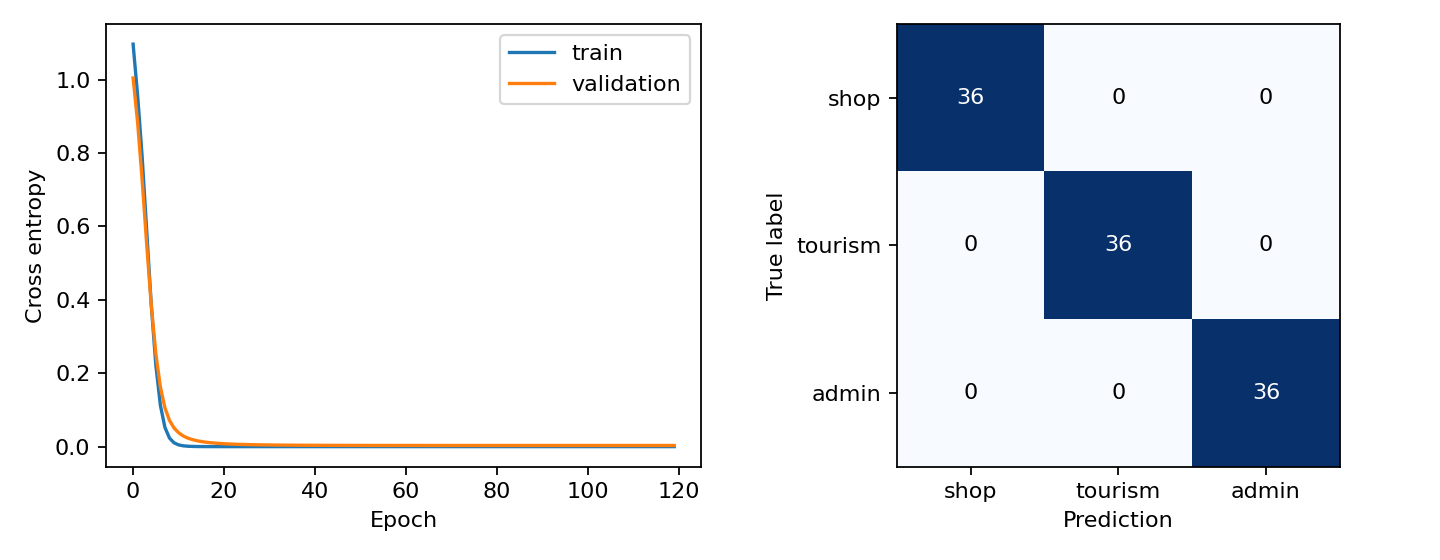
\includegraphics[width=0.98\linewidth]{results/tutorial/intent_training.png}
\captionof{figure}{Loss train/validation và confusion matrix trên 108 câu test tổng hợp.}
\end{center}

\subsection{Kết quả failure injection và
test}\label{kux1ebft-quux1ea3-failure-injection-vuxe0-test}

{\def\LTcaptype{none} % do not increment counter
\begin{longtable}[]{@{}lll@{}}
\toprule\noalign{}
Ca lỗi & Status của B1 & Số item \\
\midrule\noalign{}
\endhead
\bottomrule\noalign{}
\endlastfoot
0 & ok & 2 \\
1 & no\_results & 0 \\
2 & no\_results & 0 \\
3 & no\_results & 0 \\
4 & no\_results & 0 \\
5 & ok & 1 \\
6 & timeout & 0 \\
7 & contract\_error & 0 \\
8 & availability\_unverified & 0 \\
9 & contract\_error & 0 \\
10 & invalid\_input & 0 \\
\end{longtable}
}

Có 17 test tutorial chạy thành công; log đầy đủ nằm trong
build/tutorial\_tests.log. Hệ đã kiểm 4 lỗi bắt buộc của slide và thêm
input NaN, ID giả, sai correlation. Trường hợp OOD trong test chỉ xác
nhận câu không có token miền trả clarify, không phủ nhận các lỗi OOD đã
báo ở bảng trên.

\begin{verbatim}
python3 -m unittest discover -s tutorial -p 'test_*.py'
.................
Ran 17 tests
OK
\end{verbatim}

\subsection{Mã thực thi cần đọc khi bảo
vệ}\label{muxe3-thux1ef1c-thi-cux1ea7n-ux111ux1ecdc-khi-bux1ea3o-vux1ec7}

\lstinputlisting[firstline=68,lastline=84,caption={Deadline, xác thực envelope và trace của coordinator}]{tutorial/mas_system.py}
\lstinputlisting[firstline=85,lastline=112,caption={Luồng điều phối và trạng thái kết thúc}]{tutorial/mas_system.py}

Đoạn mã đầy đủ trong tutorial/mas\_system.py là nguồn sự thật khi cần
kiểm các dòng sau trích đoạn. Notebook thể hiện lời gọi trực tiếp, đầu
ra thực tế, dữ liệu học và các bảng kết quả; bản HTML cho phép xem
offline mà không cần chạy kernel.
